\documentclass[aspectratio=169,11pt,hyperref={colorlinks=true}]{beamer}
\usetheme{boxes}
\setbeamertemplate{navigation symbols}{}
\definecolor{ibm}{RGB}{70,107,176}
\setbeamercolor{titlelike}{fg=ibm}
\setbeamercolor{structure}{fg=ibm}
\hypersetup{colorlinks,urlcolor=ibm}
\setbeamertemplate{footline}[frame number]
% Inserting graphics
\usepackage{graphicx}
% Side-by-side figures, etc
\usepackage{subfigure}
% Code snippits
\usepackage{listings}
\usepackage{booktabs}
\usepackage{lmodern}
% Color stuff
\usepackage{color}
\usepackage{amsmath}
\usepackage{tabu}
\usepackage{amssymb}
\usepackage{empheq}
\usepackage[braket, qm]{qcircuit}
\usepackage{tikz}
\usetikzlibrary{snakes,arrows,shapes}
\usepackage{gensymb}
\usepackage{minted}
\newcommand\RBox[1]{%
  \tikz\node[draw,rounded corners,align=center,] {#1};%
}
\usepackage{hyperref}
%\usecolortheme{buzz}
%\usecolortheme{wolverine}
%\usetheme{Boadilla}
\usepackage[T1]{fontenc}

\definecolor{mygreen}{rgb}{0,0.6,0}
\definecolor{mygray}{rgb}{0.5,0.5,0.5}
\definecolor{mymauve}{rgb}{0.58,0,0.82}

\lstset{%
  backgroundcolor=\color{white},   % choose the background color; you must add \usepackage{color} or \usepackage{xcolor}
  breakatwhitespace=false,         % sets if automatic breaks should only happen at whitespace
  breaklines=true,                 % sets automatic line breaking
  captionpos=b,                    % sets the caption-position to bottom
  commentstyle=\color{ibm},  % comment style
  extendedchars=true,              % lets you use non-ASCII characters; for 8-bits encodings only, does not work with UTF-8
  keepspaces=true,                 % keeps spaces in text, useful for keeping indentation of code (possibly needs columns=flexible)
  keywordstyle=\color{blue},       % keyword style
%  otherkeywords={*,...},           % if you want to add more keywords to the set
  numbersep=5pt,                   % how far the line-numbers are from the code
  numberstyle=\tiny\color{mygray}, % the style that is used for the line-numbers
  rulecolor=\color{black},         % if not set, the frame-color may be changed on line-breaks within not-black text (e.g. comments (green here))
  showspaces=false,                % show spaces everywhere adding particular underscores; it overrides 'showstringspaces'
  showstringspaces=false,          % underline spaces within strings only
  showtabs=false,                  % show tabs within strings adding particular underscores
  stringstyle=\color{ibm},   % string literal style
}


\setbeamerfont{caption}{series=\normalfont,size=\fontsize{6}{8}}
\setbeamertemplate{caption}{\raggedright\insertcaption\par}

\setlength{\abovecaptionskip}{0pt}
\setlength{\floatsep}{0pt}

\author[Matthew Treinish]{%
    \texorpdfstring{%
        \centering
        Matthew Treinish\\
        \href{https://github.com/mtreinish/qiskit-changes-2021}{https://github.com/mtreinish/qiskit-changes-2021}
   }
   {Matthew Treinish}
}
\date{Oct 9, 2021}

\title{What's new in Qiskit 2021}
\begin{document}

\titlepage

\section{Packaging Change}
\begin{frame}
    \frametitle{The Elements}
    \centering
    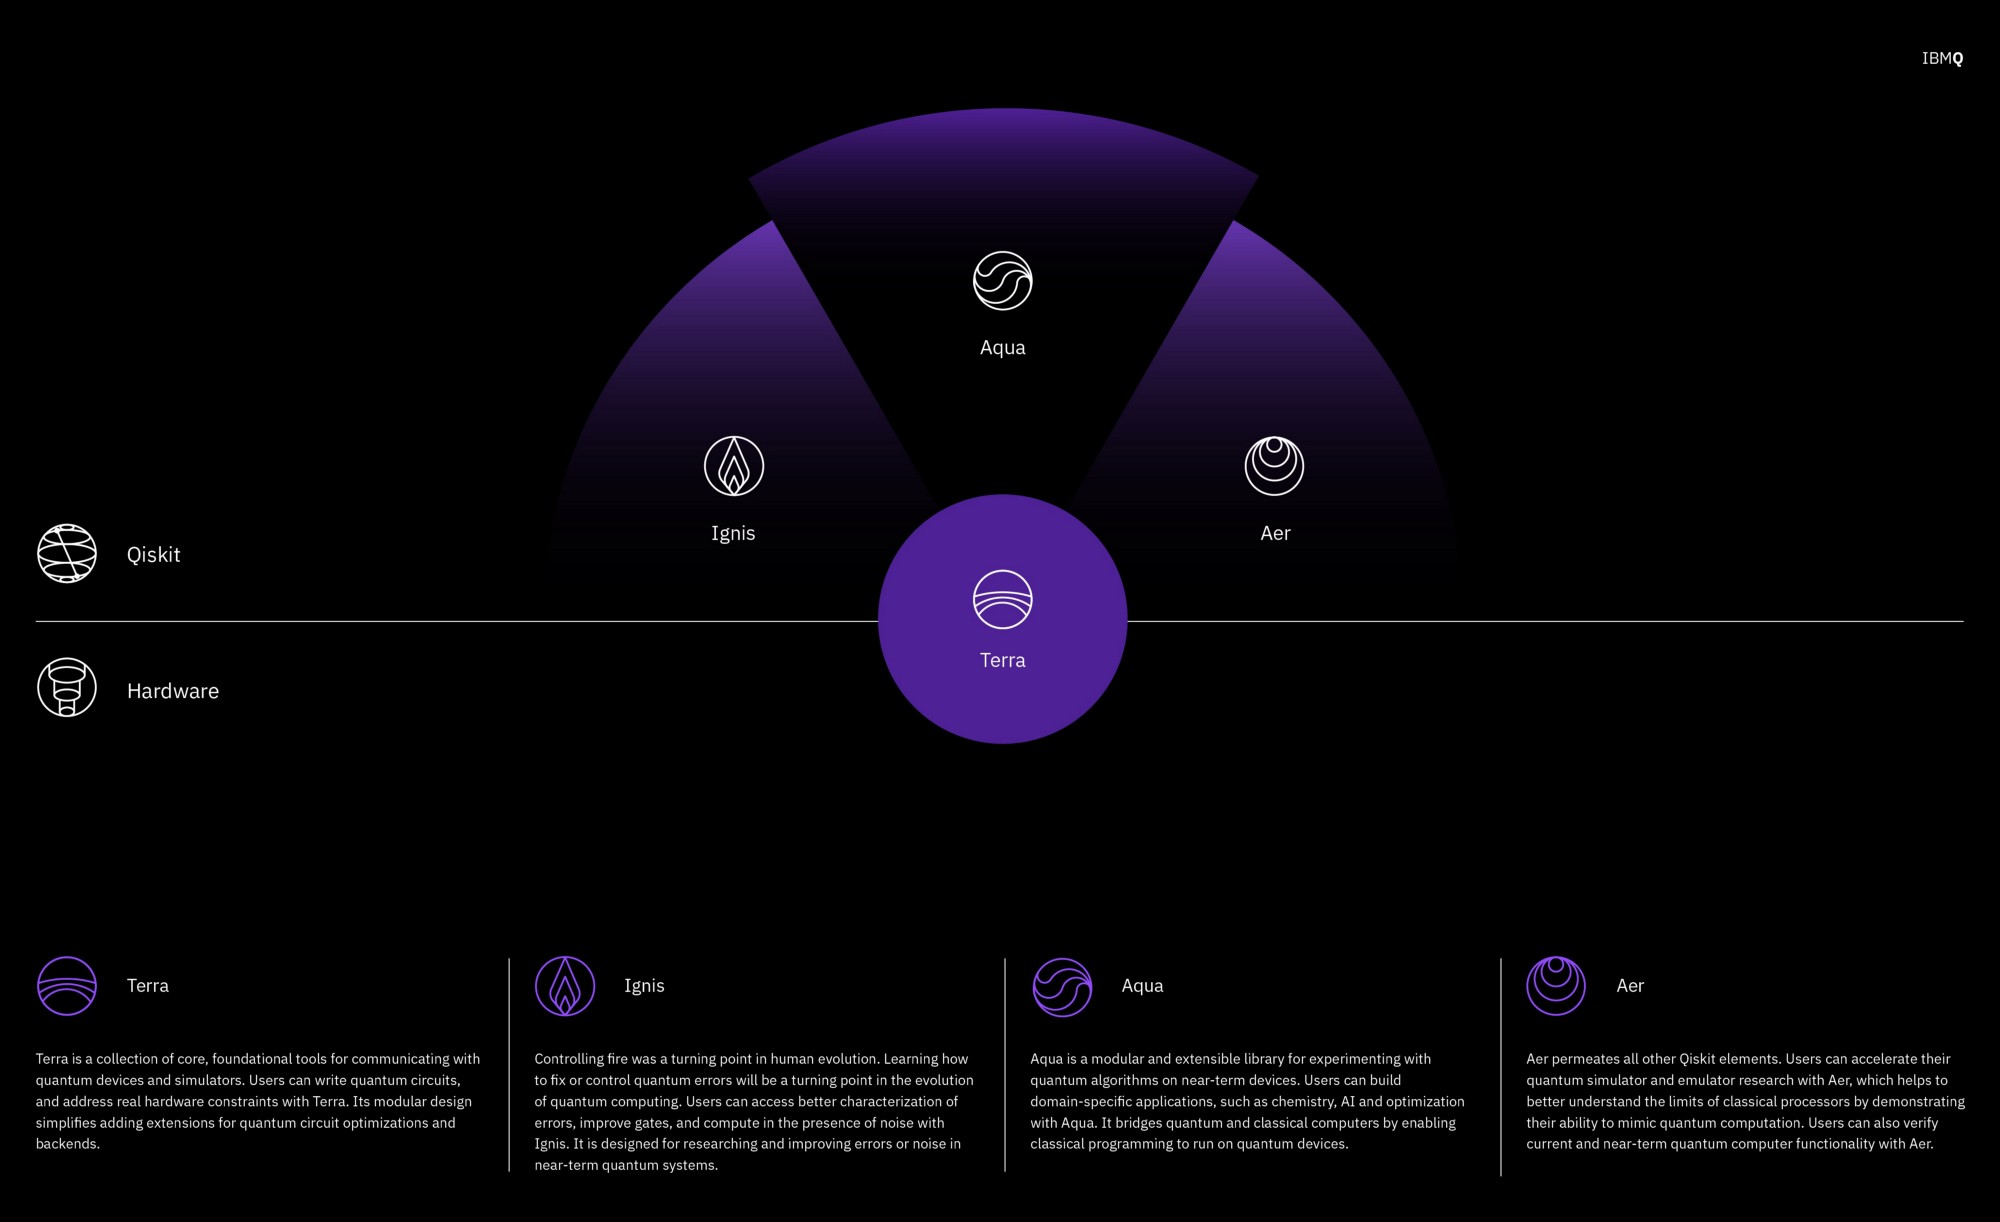
\includegraphics[width=.99\textwidth]{qiskit-components.jpeg}
\end{frame}

\begin{frame}
    \frametitle{Qiskit Moving Foward}
    \centering
    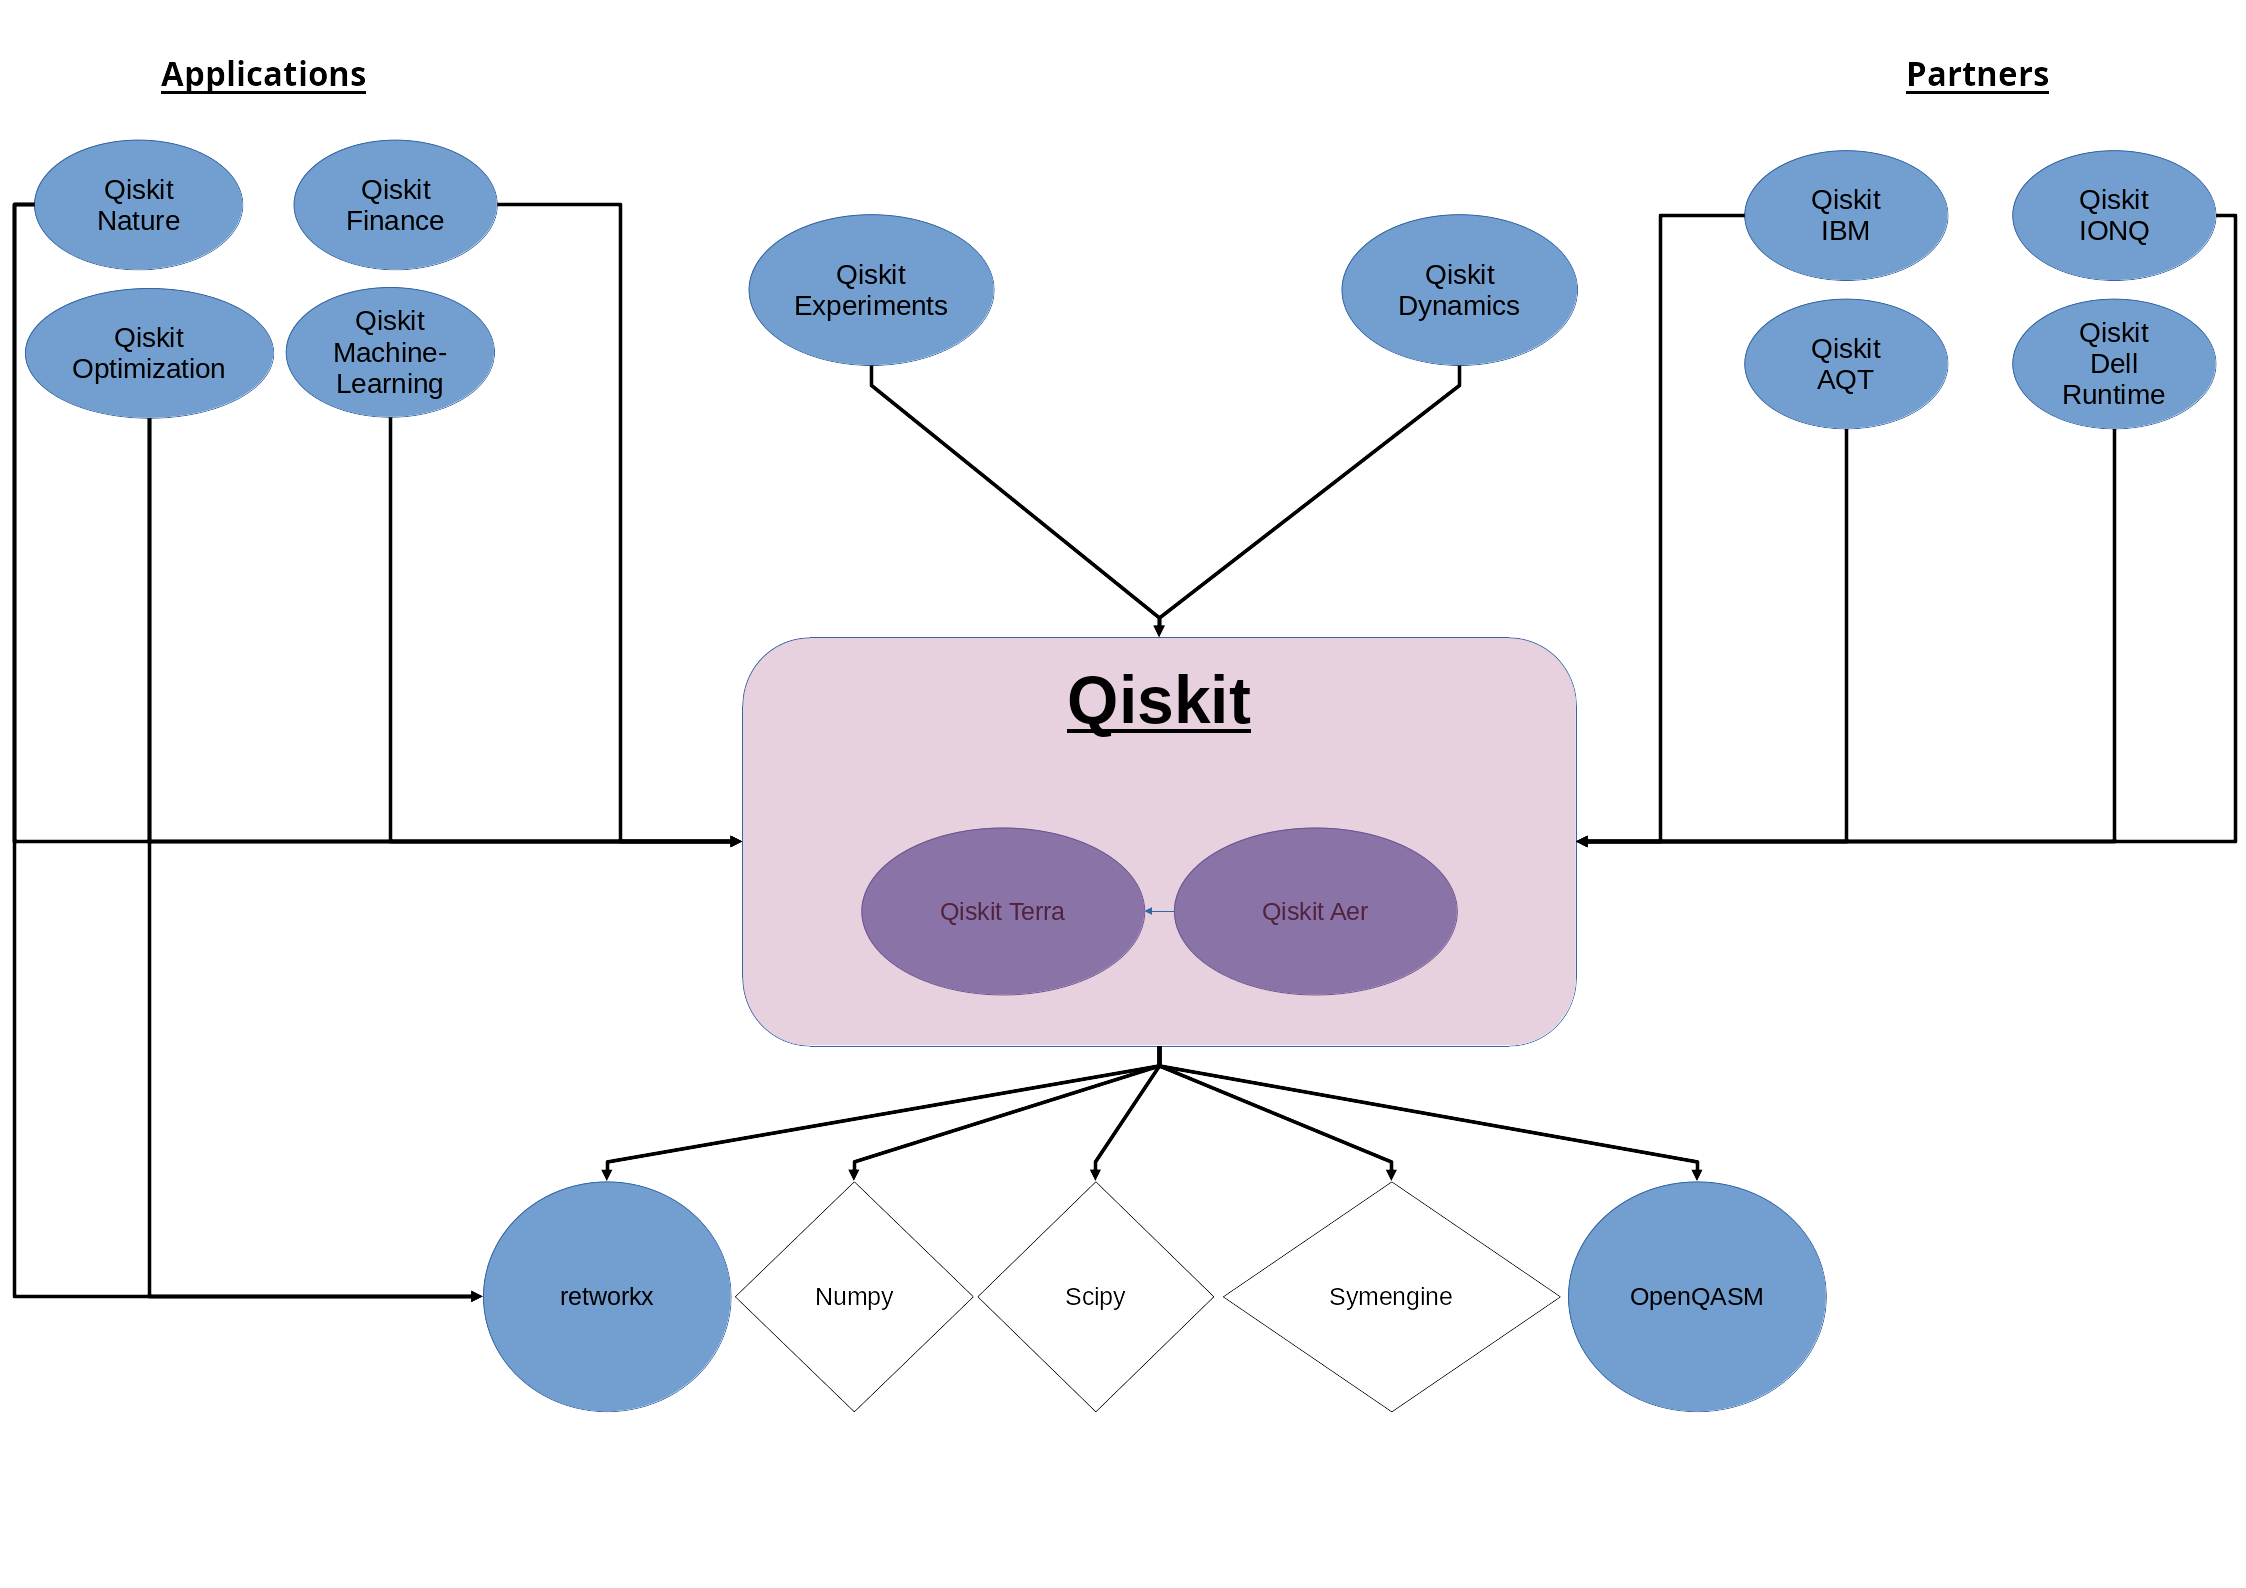
\includegraphics[width=.9\textwidth]{new_qiskit.png}
\end{frame}

\section{Qiskit Runtime}
\begin{frame}
    \frametitle{Qiskit Runtime}
    \centering
    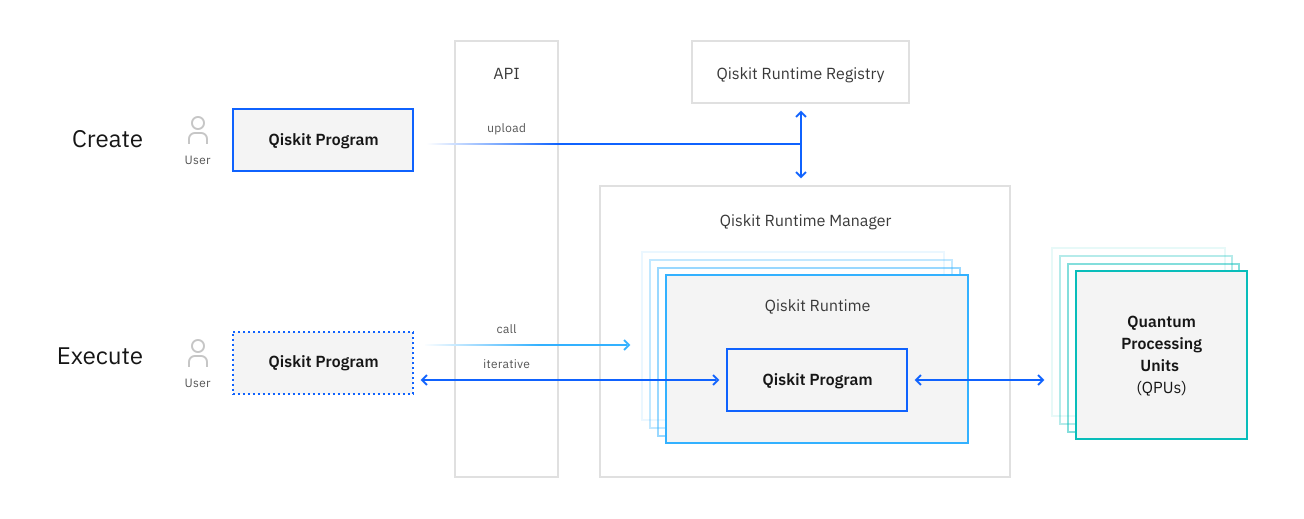
\includegraphics[width=.99\textwidth]{qiskit-runtime.png}
\end{frame}

\section{New Features}
\subsection{QPY}
\begin{frame}
    \frametitle{QPY Serialization}
    \begin{columns}
        \column{0.5\textwidth}
            \begin{itemize}
                \item Qiskit native binary serialization format for QuantumCircuit
                \item Fast serialization and deserialization for saving and
                    transfering an arbitrary number of circuits
                \item Designed to be backwards compatible moving forward (new Qiskit version can always load old QPY files generated with an older Qiskit version)
            \end{itemize}
        \column{0.5\textwidth}
            \inputminted[fontsize=\tiny]{python}{qpy_demo.py}
    \end{columns}
\end{frame}

\subsection{Improvements to backend interface}
\begin{frame}
    \frametitle{Improving the interface to backends}
    \begin{columns}
        \column{0.5\textwidth}
            \begin{itemize}
                \item Making continual improvements to Qiskit's interface with
                    hardware backends
                \item Defined a versioned interface that enables the interface
                    to change and grow in a controlled and stable/compatible
                    manner as hardware needs change
                \item Now designed to be hardware and vendor agnostic and to
                    use Qiskit objects directly
            \end{itemize}
        \column{0.5\textwidth}
            \inputminted[fontsize=\tiny]{python}{backend_demo.py} 
    \end{columns}
\end{frame}

\section{Looking to the Future}
\subsection{Control Flow}
\begin{frame}
    \frametitle{Control Flow}
    \begin{itemize}
        \item The next Qiskit release will add support for basic control flow
        \item If/else logic and for loops to start
        \item Eventually grow to support the full feature set available in QASM3
    \end{itemize}
\end{frame}

\subsection{QASM3}
\begin{frame}
    \frametitle{QASM3}
    \begin{itemize}
        \item Working on making QASM3 integrated with Qiskit
        \item Starting with support for exporting OpenQASM3 from a QuantumCircuit in the next Qiskit release
        \item Moving forward support for parsing OpenQASM3 into a QuantumCircuit
            object will be added in the future
    \end{itemize} 
\end{frame}

\section{Questions?}
\begin{frame}
\frametitle{Where to get more information}
    \begin{itemize}
        \item These Slides: \href{https://github.com/mtreinish/qiskit-changes-2021}{https://github.com/mtreinish/qiskit-changes-2021}
        \item Blog post about Qiskit restructuring: \href{https://research.ibm.com/blog/qiskit-application-modules}{https://research.ibm.com/blog/qiskit-application-modules}
        \item Qiskit Partners Documentation \href{https://qiskit.org/documentation/partners/}{https://qiskit.org/documentation/partners/}
        \item Qiskit Runtime Documentation \href{https://quantum-computing.ibm.com/lab/docs/iql/runtime/}{https://quantum-computing.ibm.com/lab/docs/iql/runtime/}
        \item Qiskit Runtime Programs \href{https://github.com/Qiskit-Partners/qiskit-runtime}{https://github.com/Qiskit-Partners/qiskit-runtime}
        \item Qiskit Release Notes \href{https://qiskit.org/documentation/release\_notes.html}{https://qiskit.org/documentation/release\_notes.html}
    \end{itemize}
\end{frame}

\end{document}
